%
\documentclass[%
 reprint,
 amsmath,amssymb,
 aps,
]{revtex4-1}

\usepackage{graphicx}% Include figure files
\usepackage{dcolumn}% Align table columns on decimal point
\usepackage{bm}% bold math


\begin{document}



\title{HERRAMIENTAS DE MAPEO OBJETO RELACIONAL (OR/M)}
\author{Orestes Ramirez Ticona}
\author{Roberto Zegarra Reyes}
\author{Orlando Acosta Ortiz}
\author{Nilson Laura Atencio}
\author{Richard Cruz Escalante}
\affiliation{%
 Universidad Privada de Tacna \textbackslash Facultad de Ingenieria \textbackslash Escuela Profesional de Ingenieria de Sistemas
}%

\begin{abstract}
\begin{center}
\textbf{Resumen}
\end{center}
En este artículo aprenderemos sobre el concepto y sus herramientas de mapeo objeto-relacional que nos permitirá crear una capa de acceso a los datos de una base de datos relacional, de tal forma que las tablas se transforman en clases y las filas de las tablas en objetos.\\
\textbf{Palabras clave:}   ORM, base de datos, herramientas, clases, objetos.\\

\begin{center}
\textbf{Abstract}
\end{center}
In this article we learn about concept and tools of Object-Relational mapping ORM that we will allow us to create an access layer to the data of a relational database, in such a way that the tables are transformed into classes and the rows of the table into objects.\\
\textbf{Keywords:}   ORM, database, tools, classes, objects.

\end{abstract}



\maketitle

%\tableofcontents

\section {Introducción}\label{sec:1}
Existen una gran variedad de herramientas para realizar el Mapeo Objeto-Relacional, ya sean libres como de pago. Algunas de estas estan ligadas al lenguaje de programacion que es orientada a objetos. Para minimizar estas dificultades de persistencia de datos, existen herramientas que se encargan de generar de manera automática el acceso a los datos, abstrayendo al programador de esta tarea. Son las llamadas herramientas ORM.
Estas herramientas que se mencionarán en el articulo, tanto para Java, .Net, PHP y Python, son una buena solucion para el desarrollo de aplicaciones de programacion orientadas a objetos (POO). 
El aprendizaje del lenguaje de la herramienta ORM puede ser algo complejo ya que, para poder sacar el máximo provecho a la herramienta, es necesario conocer en profundidad cómo funciona la misma.


%-----------------------------------------------------------------
\section{Objetivos}\label{sec:2}
\subsection{General:}
-  Permite la transformación de las tablas de una base de datos, en una serie de entidades que simplifiquen las tareas básicas de acceso a los datos para el programador.
\subsection{Específicos:}
- El mapeo relacional de objetos reduce su código de programación y, a través del almacenamiento en caché, mejora el rendimiento mediante el uso de una interfaz de SQL integrada o de nivel de llamada con un administrador de base de datos relacional. 

%-----------------------------------------------------------------
\section {Marco Teórico}\label{sec:3}
El mapeo objeto relacional es la técnica que se usa para representar un modelo orientado a objetos en una base de datos relacional, es decir, permite convertir los tipos de dato con los que trabaja un lenguaje de programación orientado a objetos a tipos de dato con los que trabaja un sistema de base de datos relacional para la persistencia de datos.
\newline
Ventajas:
\begin{itemize}
	\item Rapidez en el desarrollo: La mayoría de las herramientas actuales permiten la creación del modelo por medio del esquema de la base de datos, leyendo el esquema, nos crea el modelo adecuado.
	\item Abstracción de la base de datos: Al utilizar un sistema ORM, conseguimos separarnos del sistema de Base de datos que utilizamos.
	\item Reutilización: Utilizar los métodos de un objeto de datos desde distintas zonas de la aplicación, incluso desde aplicaciones distintas.
	\item Seguridad: Los ORM suelen implementar sistemas para evitar tipos de ataques como pueden ser los SQL injections.
	\item Mantenimiento del código: Nos facilita el mantenimiento del código debido a la correcta ordenación de la capa de datos, haciendo que sea mucho mas sencillo.
\end{itemize}
Desventajas:
\begin{itemize}
	\item Tiempo utilizado en el aprendizaje: Este tipo de herramientas suelen ser complejas por lo que su correcta utilización lleva un tiempo que hay que emplear en ver el funcionamiento correcto y ver todo el partido que se le puede sacar.
	\item Aplicaciones algo más lentas: Debido a que el sistema deberá transformar todas las consultas que se hagan sobre la base de datos al lenguaje propio de la herramienta, luego leer los registros y por último crear los objetos.
\end{itemize}

Algunas de las herramientas para la realización de Mapeos Objeto-Relacional son:

\subsection{Para Java}
\begin{itemize}
	\item Hibernate: Es una herramienta de Mapeo Objeto-Relacional para Java lo que significa que los mapeos se construyen alrededor de declaraciones de clases persistentes y no alrededor de declaraciones de tablas.\cite{Community}\\
Facilita el mapeo de atributos entre una base de datos relacional tradicional y el modelo de objetos de una aplicación, mediante ficheros declarativos (XML) que permite al desarrollador detallar cómo es su modelo de datos, qué relaciones existen y qué forma tienen. Hibernate está diseñado para ser flexible en cuanto al esquema de tablas utilizado, para poder adaptarse a su uso sobre una base de datos ya existente. También tiene la funcionalidad de crear la base de datos a partir de la información disponible.\cite{JuntaAndalucia}\\
Caracterísiticas:\\
- Modelo de programación natural\\
- Gran escalabilidad\\
- Software libre\\
- Persistencia transparente, ofrece soporte para un amplio conjunto de las colecciones de Java.\\
- Mapeado flexible gracias a las asociaciones bidireccionales\\
- Facilidades en consultas y metadatos
	\item iBatis: Es un framework mapeador de datos que provee unos medios muy simples y flexibles de cambiar de lugar los datos entre sus objetos de Java y una BBDD relacional. En realidad, iBatis no es un verdadero ORM (Mapeo Objeto Relacional), sino que en iBatis el SQL se tendrá que escribir por uno mismo, en comparación con Hibernate que genera el SQL para mapear objetos a tablas de la base de datos. \cite{Batis}\\
Propone un modelo de objetos inerte en donde las distintas operaciones de borrado, modificación, lectura, etc. sobre estos deben ser trasladados a la base de datos y viceversa. Mapea propiedades de objetos a parámetros para las PreparedStatement (sentencias SQL parametrizables) y mapea los resultados de una query a un objeto o una lista de objetos.
	\item Torque: Torque es una capa de persistencia, permite evitar la codificación directa de SQLs, así como abstraer al programador de la problemática vinculada con la apertura y cierre de conexiones a BBDD, siendo también adaptable a diferentes SGBD para crear un modelo físico de datos. El Torque incluye un generador para generar todos los recursos de base de datos requeridos por su aplicación e incluye un ambiente de tiempo de ejecución para dirigir las clases generadas. \cite{Torque}\\
\end{itemize}
\subsection{Para .Net}
\begin{itemize}
	\item NHibernate: según su website es: "NHibernate es un maduro , de código abierto mapeador objeto-relacional para el marco .NET. Está desarrollado de forma activa , con todas las funciones y se utiliza en miles de proyectos exitosos."\cite{nhibernate}

Hibernate es bastante antiguo y es utilizado por miles de aplicaciones de productos, NHibernate no solo ha heredado la mayoría de las buenas características de su antecesor de Java, sino que también se ha enriquecido con características de .NET, como las consultas LINQ. Las consultas LINQ (consulta integrado al lenguaje) ofrece consultas de datos y sistanxis actualizada, la cual es similar a SQL.
NHibernate tiene muchas de estas características que harán que escribir código de interacción de base de datos sea muy fácil. Es un proyecto de código abierto que prospera enteramente en las contribuciones de la comunidad..\cite{chatekar2015}\\
Caracterísiticas:\\
- Comunidad establecida\\
- Ciclo de desarrollo rápido\\
- Toneladas de complementos y herramientas de búsqueda de texto completo.\\
- Fácil para Visual Studio Asigne
	\item Entity Framework: es el puente que une naturalmente ambos lados. Entity Framework ofrece un entorno estable para mapear una base de datos relacional de manera bastante eficiente. Titulary Los marcos de trabajo cargan los datos, tablas y relaciones automáticamente desde la base de datos real, sin necesidad de declarar objetos y variables previamente .\cite {ef} \\
\begin{figure}[htb]
\begin{center}
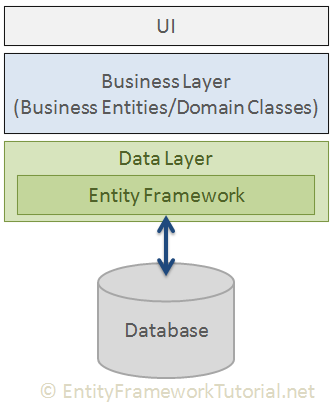
\includegraphics[width=5cm]{./Imagenes/ef}
\end{center}
\end{figure}
 Entity Framework se ajusta entre las entidades comerciales (clases de dominio) y la base de datos. Guarda los datos almacenados en las propiedades de las entidades comerciales y también recupera datos de la base de datos y los convierte en objetos de entidades comerciales de forma automática.\\
\\
\\
\\
\\
\\
	\item DataObjects.NET: es un marco de mapeo de persistencia y relacional de objetos para Microsoft .NET. Permite a los desarrolladores definir objetos persistentes y lógica de negocios directamente en C\#, Visual Basic. Los objetos persistentes pueden ser recuperados por consultas LINQ. Los datos persistentes se pueden almacenar en servidores SQL. A diferencia de muchos otros marcos ORM, el modelo de base de datos se genera y mantiene automáticamente.\cite{do} \\
\end{itemize}
\subsection{Para PHP}
\begin{itemize}
	\item Doctrine Project : es un conjunto de librerías PHP entre las que se encuentra ORM. Doctrine 1 comenzó en 2006, pero hasta finales de 2010 no se lanzó Doctrine 2, una versión muy mejorada respecto a la anterior. Las entidades en Doctrine 2 son objetos PHP que contienen variables (propiedades) que se guardan y devuelven a una base de datos a través del Entity Manager de Doctrine, una implementación del patrón de mapeador de datos. Su principal característica es la poca configuración que hace falta para empezar un proyecto.\cite{doct}\\
	\item Propel: Es un Mapeo Relacional (ORM) de código abierto para bases de datos SQL en PHP 5.5. Le permite acceder a su base de datos utilizando un conjunto de objetos, proporcionando una API simple para almacenar y recuperar datos.\\
Además de sus capacidades ORM, proporciona un generador de consultas , migración de esquema de base de datos , ingeniería inversa de la base de datos existente y mucho más.\\
Utiliza PDO como capa de abstracción y generación de código para eliminar la carga de la introspección en tiempo de ejecución para lograr un tiempo de ejecución rápido.\\
Propulsar implementos de todos los conceptos clave de capas maduras ORM: el ActiveRecord patrón, validadores , comportamientos , herencia de tablas , realizar ingeniería inversa en una base de datos existente , conjuntos anidados , transacciones anidadas , la carga diferida , LOB , lo que sea.\\
Propel está diseñado para desarrolladores que necesitan mantener el control de su código:\\
- La extensibilidad está en el corazón del diseño de Propel; Cualquier cosa que necesite personalizar, Propel le permite hacerlo en un instante.
- Propel puede salirse de su camino cuando necesita consultas personalizadas o transacciones hiper-optimizadas.
- Si necesita cambiar su RDBMS en el curso del proyecto, reconstruya su modelo y estará listo para comenzar. Propel soporta MySQL, PostgreSQL, SQLite, MSSQL y Oracle. Los tres primeros están completamente integrados en nuestra suite de pruebas.
- El código generado por Propel está bien comentado, es compatible con IDE y es fácil de usar.\\
El proyecto Propel comenzó en 2005 y ya alimenta miles de sitios web. Completamente documentado, respaldado por muchos tutoriales en la web, también se beneficia de una comunidad entusiasta que brinda soporte rápido para desarrolladores tanto principiantes como incondicionales. Propel se lanza bajo la licencia MIT . Es de uso gratuito, incluso en aplicaciones comerciales.\cite{propel}\\
	\item Torpor : Es un marco de Mapeo Relacional de Objetos (ORM) y una abstracción de la capa de persistencia para PHP, que se caracteriza por las siguientes características:\\
- Facilidad de instalación, configuración y extensión.\\
- Fábricas de objetos ligeros y definición de clase sobre la marcha.\\
- Obtención justo a tiempo y operaciones masivas eficientes.\\
- Almacenamiento en caché intermedio de lectura / escritura en subprocesos, sesiones o niveles de red distribuidos.\\
- Fábricas de objetos relacionados, carga profunda y dependencia de recursión segura en cascada para publicación.\\
- Arquitectura de plug-in e interfaces para la abstracción de la base de datos con soporte listo para usar para:\\
   - MySQL\\
   - Microsoft SQL Server\\
   - Oracle\\
   - SQLite
	Torpor utiliza una configuración XML validada por esquema (que puede opcionalmente producirse automáticamente usando las herramientas incluidas) para describir un repositorio de datos, y actúa como una fábrica inteligente para crear objetos correspondientes a estructuras de datos, completos con mutadores adecuados y accesos directos convenientes para una carga profunda (recuperación) de objetos relacionados). Se puede utilizar una amplia variedad de criterios para la búsqueda de objetos, aplicados no solo a los datos deseados, sino a cualquier clase de datos a los que hace referencia, o que se refieren a ellos, asociados automáticamente por el motor de datos y con una selección de ruta más corta estrechamente controlada rutinas (uniones ANSI exclusivas y bien formadas, en el caso de SQL). También se proporcionan operaciones en masa de toda la colección (recuperación de objetos múltiples dentro de una sola transacción) y paginación del lado de la base de datos.\cite{torpor}\\
\end{itemize}

\subsection{Para Phyton}
La capacidad de escribir código Python en lugar de SQL puede acelerar el desarrollo de aplicaciones web, especialmente al comienzo de un proyecto. El potencial aumento de la velocidad de desarrollo proviene de no tener que cambiar del código de Python a la escritura de sentencias de SQL de paradigma declarativo.\cite{Phyton}
\begin{itemize}
	\item SQLObject:es fácil de usar, es independiente de la base de datos y puede hacer las tablas por nosotros. 
	\item  Django:ORM tiene una sintaxis más limpia y es más fácil escribir para (patrón ActiveRecord),también tiene una capa declarativa que oculta cierta complejidad y le da una sintaxis de estilo ActiveRecord más similar a la ORM de Django.
	\item  Peewee ORM:Peewee es una implementación ORM de Python que está escrita para ser " más simple, más pequeña y más hackeable " que SQLAlchemy. 
           \item SQLAlchemy:es más completo y potente (usa el patrón DataMapper), a la vez También se integra a la perfección con las clases / tablas configuradas usando el estilo de intercambio de datos, Pero las cosas se vuelven muy complejas si hay muchas relacion ademas SQLAlchemy soporta OOP y estilos funcionales listos para usar,Si bien es cierto es muy poderoso. Sin embargo, no es seguro para subprocesos.
          \item ponyorm:es un ORM (Object Relational Mapper) escrito en Python puro. Ofrece una sintaxis de comprensión de lista fácil de usar para consultar objetos,tambien puede concentrarse en escribir la lógica de negocios de su aplicación y usar la sintaxis de Python para interactuar con la base de datos. Pony traduce dichas consultas a SQL y las ejecuta en la base de datos de la manera más eficiente.\cite{poni}

\end{itemize}


%-----------------------------------------------------------------
\section{Ejemplo}\label{sec:4}

En nuestro ejemplo usaremos la herramienta de Entity Framework.\\
\begin{itemize}
	\item En nuestra solucion SistemaGYM, tenemos dos proyectos que necesitamos para el mapeo.
		\begin{figure}[htb]
\begin{center}
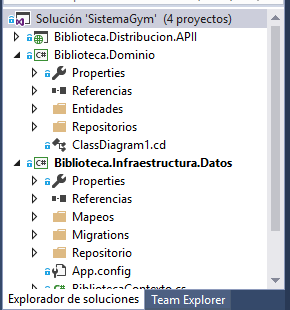
\includegraphics[width=5cm]{./Imagenes/1}
\end{center}
\end{figure}

	\item En el proyecto Biblioteca.Dominio, donde se encuentra la capa de entidades.
\begin{figure}[htb]
\begin{center}
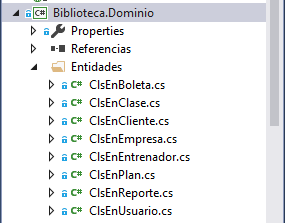
\includegraphics[width=5cm]{./Imagenes/2-1}
\end{center}
\end{figure}

	\item En cada clase se especifican los atributos y sus relaciones.
\begin{figure}[htb]
\begin{center}
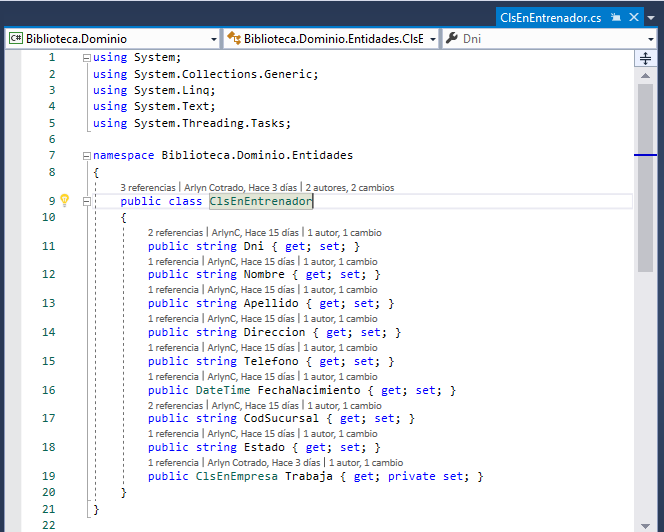
\includegraphics[width=7cm]{./Imagenes/2-2}
\end{center}
\end{figure}
\\

	\item En el proyecto Biblioteca.Infraestructura.Datos, donde se encuentran las tablas, relaciones y llaves.
\begin{figure}[htb]
\begin{center}
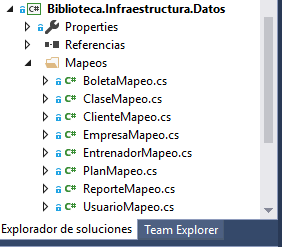
\includegraphics[width=6cm]{./Imagenes/3}
\end{center}
\end{figure}
\begin{figure}[htb]
\begin{center}
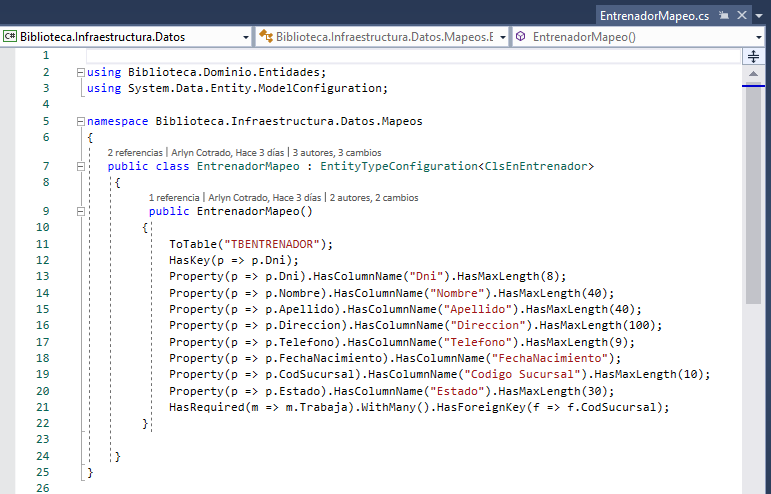
\includegraphics[width=9cm]{./Imagenes/3-1}
\end{center}
\end{figure}
\\
\\
\\
\\
\\
\\
\\
\\
\\
\\
\\
\\
\\
\\
\\
\\
\\
\\
	\item Creamos el contexto de la base de datos.
\begin{figure}[htb]
\begin{center}
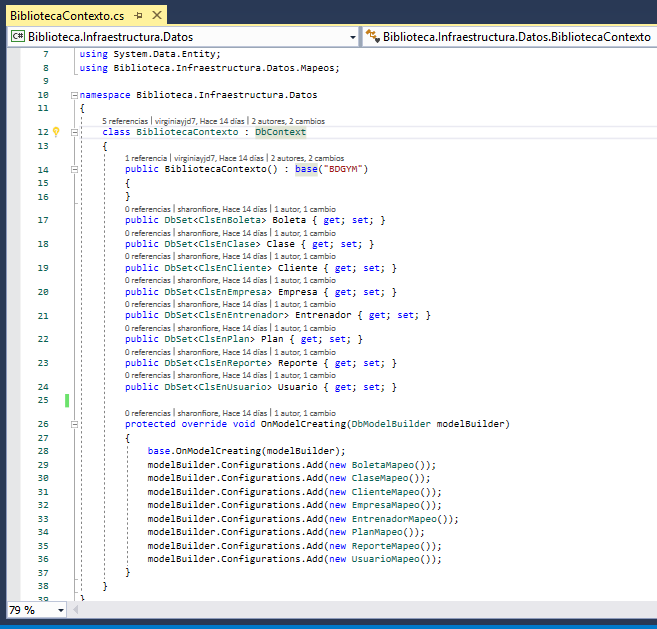
\includegraphics[width=9cm]{./Imagenes/4}
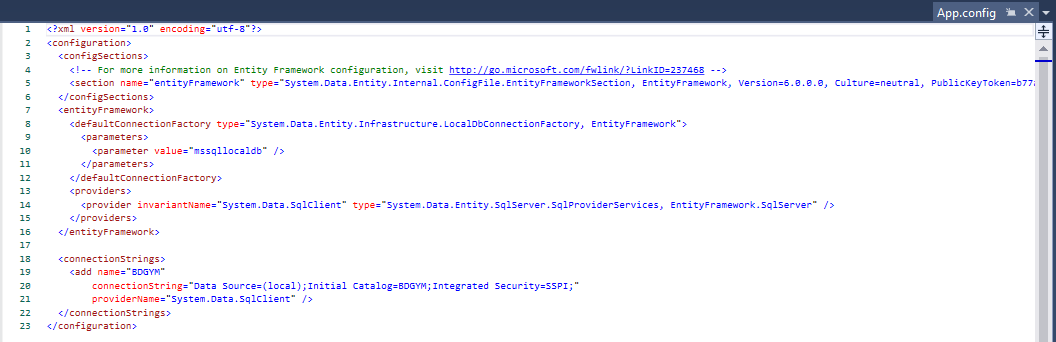
\includegraphics[width=9cm]{./Imagenes/4-1}
\end{center}
\end{figure}\\
\\
\\
\\
\\
\\
\\
	\item Abrimos la Consola del Administrador de paquetes. Ingresamos los siguientes comandos: Enable-Migrations, add-migration, Update-Database.\\
\begin{figure}[htb]
\begin{center}
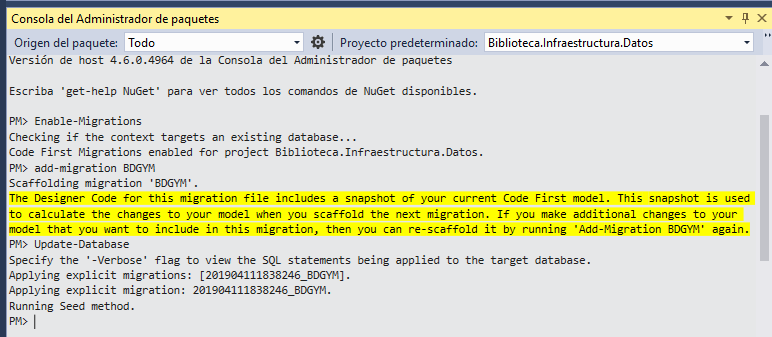
\includegraphics[width=9cm]{./Imagenes/5-1}
\end{center}
\end{figure}
\\
\\
\\
\\
\\
\\
\\
	\item Por ultimo, vemos la base de datos, para ello entramos a SQL Server.
\begin{figure}[htb]
\begin{center}
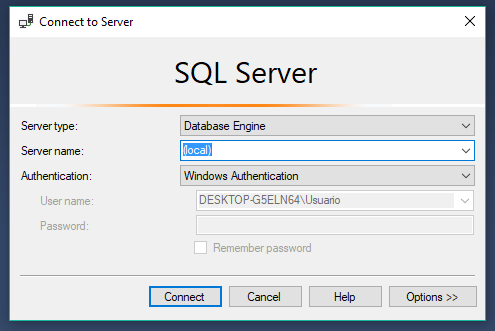
\includegraphics[width=6cm]{./Imagenes/5}
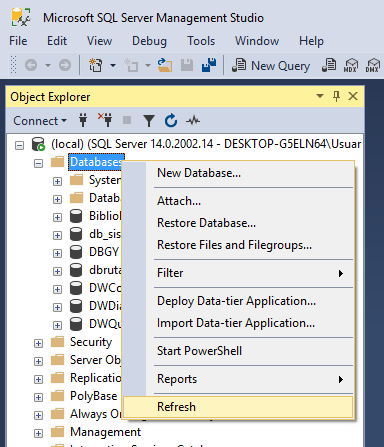
\includegraphics[width=6cm]{./Imagenes/5-2}
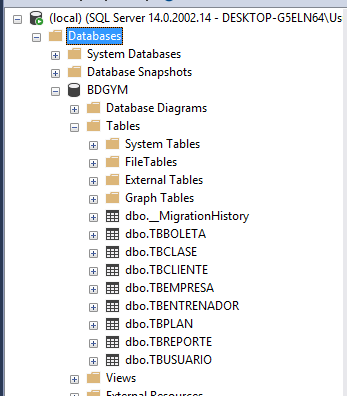
\includegraphics[width=6cm]{./Imagenes/5-3}
\end{center}
\end{figure}
\\
\\
\\
\\
\\
\\
\begin{figure}[htb]
\begin{center}
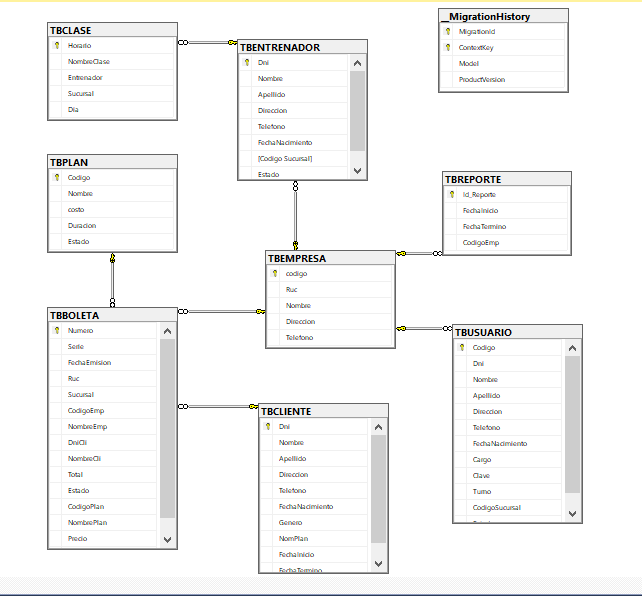
\includegraphics[width=9cm]{./Imagenes/6}
\end{center}
\end{figure}

\end{itemize}

%-----------------------------------------------------------------
\section {Análisis}\label{sec:5}
-Los ORM proporcionan una abstracción de alto nivel en una base de datos relacional que permite a un desarrollador escribir código Python en lugar de SQL para crear, leer, actualizar y eliminar datos y esquemas en su base de datos. Los desarrolladores pueden usar el lenguaje de programación con el que se sienten cómodos para trabajar con una base de datos en lugar de escribir sentencias de SQL o procedimientos almacenados.

\section{Conclusiones}\label{sec:6}


\begin{itemize}
	\item El mapeo objeto-relacional (ORM) es una técnica para mapear sistemas orientados a objetos a bases de datos relacionales.
	\item Utilizar las diferentes herramientas de ORM, da mas rapidez y eficiencia a la construcción de base de datos.
\end{itemize}


% Bibliografia.
%-----------------------------------------------------------------

\bibliographystyle{plain}
\bibliography{Bibliografia}

\end{document}
